\documentclass{article}

\usepackage{amsmath}
\usepackage{amssymb}
\usepackage{multicol}
\usepackage{graphicx}
\usepackage{gensymb}
\usepackage{esint}
\usepackage{booktabs}
\usepackage{dsfont}

\graphicspath{ {./img/} }

%title page
\title{Math}
\date{2021-02-06}
\author{Nicholas Huber}

\begin{document}
  \maketitle
  \newpage
  \tableofcontents
  \newpage

\section{\underline{Exponents}}
\begin{itemize}
  \item Multiply some number many times
  \item $b^{n}$
  \item $b$\ the base
  \item $n$\ the exponent or power of $b$
  \item $\exp(x)\equiv e^{x}$: exponential function base $e$
  \item Properties:
    \begin{itemize}
      \item Multiplying two expressions with like-bases: $b^{m}b^{n}\ \equiv\ b^{m+n}$
      \item Division can be expressed in the following way: $b^{-1}\ \equiv\ \frac{1}{b}$
      \item $\frac{b^{m}}{b^{n}}\ \equiv\ b^{m-n}$
      \item $(b^{m})^{n}\ \equiv\ b^{mn}$
      \item $(ab)^{n}\ \equiv\ a^{a}b^{n}$
      \item $\left(\frac{a}{b}\right)^{n}\ \equiv\ \frac{a^{2}}{b^{n}}$
      \item $b^{\frac{1}{n}}\ \equiv\ \sqrt[\leftroot{-3}\uproot{3}n]{b}$
      \item $\sqrt[\leftroot{-3}\uproot{3}n]{ab}\ \equiv\ (ab)^{\frac{1}{n}}\ \equiv\ a^{\frac{1}{n}}b^{\frac{1}{n}}\ \equiv\ \sqrt[\leftroot{-3}\uproot{3}n]{a}\sqrt[\leftroot{-3}\uproot{3}n]{b}$
      \item $\sqrt[\leftroot{-3}\uproot{3}n]{\left(\frac{a}{b}\right)}\ \equiv\ \left(\frac{a}{b}\right)^{\frac{1}{n}}\ \equiv\ \frac{a^{\frac{1}{n}}}{b^{\frac{1}{n}}}\ \equiv\ \frac{\sqrt[\leftroot{-2}\uproot{2}n]{a}}{\sqrt[\leftroot{-1}\uproot{1}n]{b}} $
    \end{itemize}
\end{itemize}

\section{\underline{Logarithms}}
\begin{itemize}
  \item Inverse of eponentiation
  \item $\log_{b}(x)$:\ $\log$\ of $x$\ base $b$\ is the inverse of $b^{x}$
  \item $\log_{b}(x) = m\ \Leftrightarrow\ b^{m}\ =\ x$
  \item $\ln(x)$:\ the natural log; a log with base $e$; inverse of $e^{x}$
  \item $\log(x)+\log(y) = \log(xy)$
  \item $\log(x^{k})j = k \log(x)$
  \item $\log(x)-\log(y) = \log\left(\frac{x}{y}\right)$
  \item $\log_{B}(x)\ =\ \frac{\log_{b}(x)}{\log_{b}(B)}$
  \item $\log_{10}(S)\ =\ \frac{\log_{10}(S)}{1}\ =\ \frac{\log_{10}(S)}{\log_{10}(10)}\ =\ \frac{\log_{2}(S)}{\log_{2}(10)}\ =\ \frac{\ln(S)}{\ln(10)}$
\end{itemize}


\section{\underline{Polynomials}}

\begin{equation*}
  f(x) = ax^2 + bx + c
\end{equation*}
\begin{itemize}
\item Degree of $f(x)$ is the largest power of $x$.
\item Roots of $f(x)$ are the values of $x$ for which $f(x) = 0$.
\item A polynomial of \textit{n}th degree can be written using summation.
\end{itemize}

\begin{equation*}
  f(x) = a_{n}x^{n} + a_{n-1}x^{n-1} + ... a_{2}x^{2} + a_{0}
\end{equation*}
\begin{equation*}
  f(x) = \sum_{k=0}^{n} a_{k}x^{k}
\end{equation*}

\subsection{\underline{Solving Polynomials}}
\begin{itemize}
  \item First degree polynomials\\
  \begin{align*}
    P_{1}(x) &= mx + b = 0\\
    x &= \frac{b}{m}
  \end{align*}
  \item Second degree polynomials\\
  \begin{align*}
    P_{2}(x) &= ax^{2} + bx + c = 0\\
    x_{1} &= \frac{-b+\sqrt{b^{2}-4ac}}{2a}\\
    x_{2} &= \frac{-b-\sqrt{b^{2}-4ac}}{2a}\\
  \end{align*}
  If $b^{2} - 4ac < 0$, it involves taking the square root of a negative number, for which no real solution exists.
\end{itemize}

\subsection{\underline{Polynomial Example}}
The revenue of a company: $R(x)$\\
The cost incurred: $C(x)$\\
The cost to break even: $R(x) = C(x)$\\

\begin{multicols}{2}
  \begin{align*}
    R(x) &= 2x^{2} + 2x\\
    C(x) &= x^{2} + 5x + 10\\
    2x^{2} + 2x &= x^{2} + 5x + 10\\
  \end{align*}
  \begin{align*}
    2x^{2} + 2x &= x^{2} + 5x + 10\\
    x^{2} + 2x &= 5x + 10\\
    x^{2} - 3x &= 10\\
    x^{2} -3x - 10 &= 0\\
  \end{align*}
\end{multicols}
\[  a = 1  b = -3  c = -10 \]
\begin{multicols}{2}
\begin{align*}
  x_{1} &= \frac{-b + \sqrt{b^{2} - 4ac}}{2a}\\
  x_{1} &= \frac{3 + \sqrt{9 - 40}}{2}\\
  x_{1} &= \frac{3 + 7}{2}\\
  x_{1} &= \frac{10}{2}\\
  x_{1} &= 5\\
\end{align*}

\begin{align*}
  x_{2} &= \frac{-b - \sqrt{b^{2} - 4ac}}{2a}\\
  x_{2} &= \frac{3 - \sqrt{9 + 40}}{2}\\
  x_{2} &= \frac{3 - 7}{2}\\
  x_{2} &= \frac{-4}{2}\\
  x_{2} &= -2\\
\end{align*}
\end{multicols}

\section{\underline{Trigonometry}}

%\begin{figure}[ht]
%  \caption{Trigonometric Identities}
%  \label{fig:circle1}
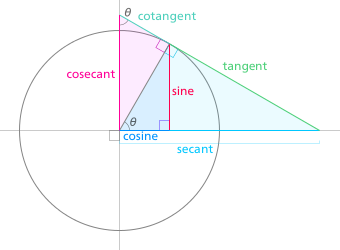
\includegraphics[width=\linewidth]{trig.png}
%\end{figure}

\subsection{\underline{Basic Concepts}}
\begin{itemize}
  \item A, B, C: three vertices
  \item $\theta$: angle
  \item $opp \equiv \overline{AB}$: the length of the side opposite $\theta$.
  \item $adj \equiv \overline{BC}$: the length of the side adjacent $\theta$.
  \item $hyp \equiv \overline{AC}$: the length of the longest side (hypotenuse)
  \item \textit{h}: the height of the triangle.
  \item $\sin\theta\equiv\frac{opp}{hyp}$: the sine of theta is the ratio of the length of the opposite side and the hypotenuse.
  \item $\cos\theta\equiv\frac{adj}{hyp}$: the cosine of theta is the ratio of the length of the adjacent side and the hypotenuse.
  \item $\tan\theta\equiv\frac{\sin\theta}{\sin\theta} \equiv \frac{opp}{adj}$: the tangent is the ratio of the opposite length divided by the adjacent length.
\end{itemize}

\subsubsection{Pythagorean Theorem}
The length of the hypotenuse squared is equal to the sum of the squares of the lengths of the opposite and adjacent sides:
\begin{itemize}
  \item $|adj|^{2} + |opp|^{2} = |hyp|^{2}$
  \item $\frac{|adj|^{2}}{|hyp|^{2}} + \frac{|opp|^{2}}{|hyp|^{2}} = 1$
  \item $\cos^{2}\theta + \sin^{2}\theta = 1$
\end{itemize}


\subsection{\underline{Radians}}
Radians are the natureal unit for measurings angles.
\begin{itemize}
  \item $2\pi = 360\degree$
  \item If a circle has a radius $r = 1$, then the arc length is equal to the angle in radians $\ell$.  $\ell = \theta_{rad}$.
  \item Measuring radians is equivalent to measuring arc length on a circle of radius 1.
\end{itemize}

\subsection{\underline{Unit Circle}}
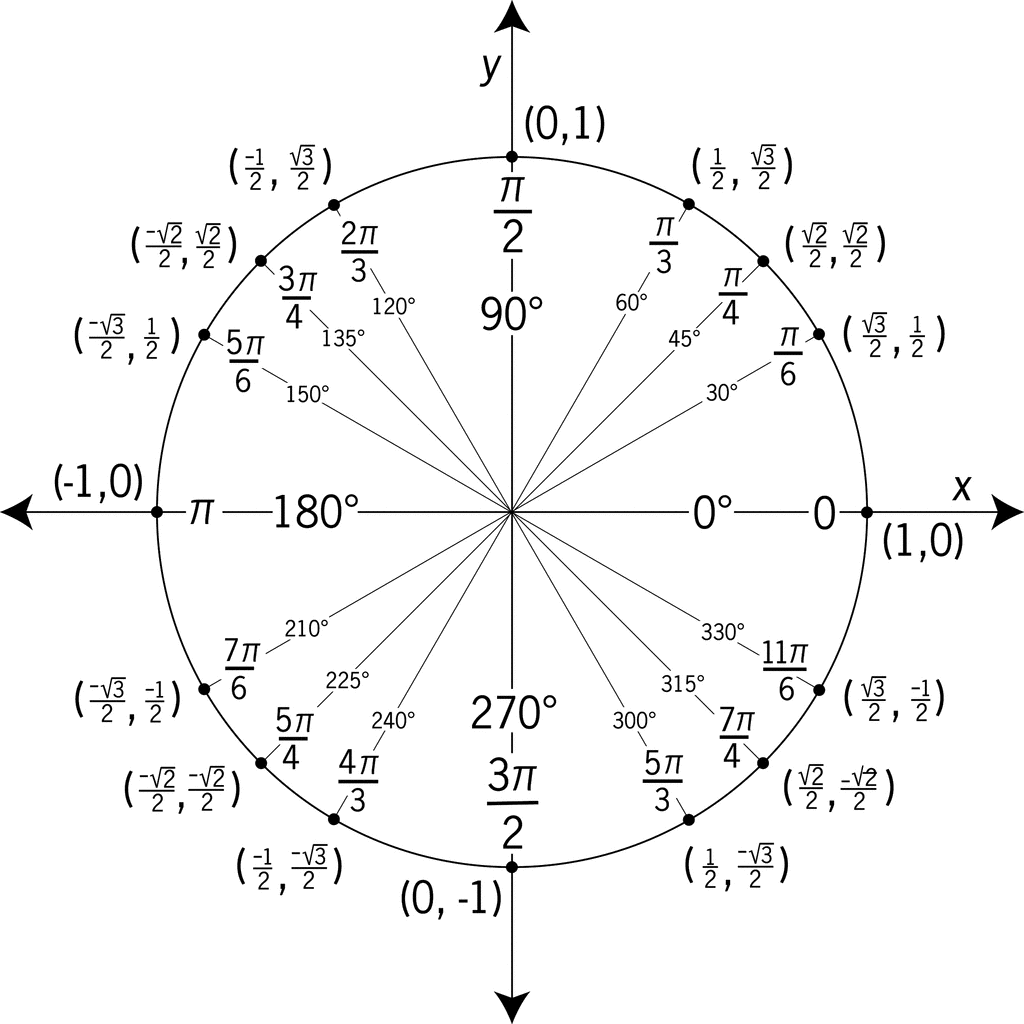
\includegraphics[width=\linewidth]{unitcircle1.png}
\begin{itemize}
  \item Length of radius is equal to 1.
  \item $P =$ a point on the unit circle
  \item $P(\theta) = (P_{x}(\theta), P_{y}(\theta)) = (\cos\theta, \sin\theta)$
\end{itemize}
\subsubsection{Polar Coordinates}
\begin{itemize}
  \item Used for circles
  \item $r\angle\theta$ $r =$ radius, $\angle\theta =$ the angle from the x axis
  \item Given the form $(r, \theta)$
  \item Example: $\left(2, \frac{\pi}{6}\right)$
\end{itemize}
\subsection{\underline{Sine and Cosine}}
\begin{itemize}
  \item Take angles as inputs and output ratios
  \item Sine: How tall a triangle is
  \item Cosine: How wide a triangle is
  \item $\cos^{2}\theta + \sin^{2}\theta = 1$ for all angles.
  \item Knowing that $\sin(30\degree) = \sin\left(\frac{\pi}{6}\right) = \frac{1}{2}$ and the previous rule you can determine all other angles.
  \begin{align*}
    \cos(30\degree) =& \sqrt{1 - \sin^{2}(30\degree)}\\
                    =& \sqrt{1 - \frac{1}{4}}\\
                    =& \sqrt{\frac{3}{4}}\\
                    =& \frac{\sqrt{3}}{2}
  \end{align*}
  \item For non unit circles: $Q(\theta) = (Q_{x}(\theta), Q_{y}(\theta)) = (r \cos\theta, r \sin\theta)$
\end{itemize}

\subsubsection{Trigonometric Identities}
\begin{itemize}
  \item sico + sico: $\sin(a + b) = \sin(a)\cos(b) + \sin(b)\cos(a)$
  \item coco - sisi: $\cos(a + b)  \cos(a)\cos(b) - \sin(a)\sin(b)$
\end{itemize}
\subsubsection{Derived Formulae}
Using the above Identities, the following can be derived:
\begin{itemize}
  \item Double angle formulae:
    \begin{align*}
      \sin(2x) &= 2\sin(x)\cos(x)\\
      \cos(2x) &= 2\cos^{2}(x) - 1\\
               &= 2(1 - sin^{2}(x)) - 1\\
               &= 1 - 2\sin^{2}(x)
    \end{align*}
  \item The above could also be rewritten as:
    \begin{multicols}{2}
      \begin{equation*}
        \cos^{2}(x) = \frac{1}{2}(1 + \cos(2x))\\
        \qquad\sin^{2}(x) = \frac{1}{2}(1 - \cos(2x))
      \end{equation*}
    \end{multicols}
  \item Self similarity
    \begin{itemize}
      \item Sine and Cosine are periodic functions with a period of $2\pi$, adding a multiple of $2\pi$ to the input has no change to the function.
      \item Sine and Cosine are $\frac{\pi}{2}$ shifted versions of each other:
      \begin{multicols}{2}
        \begin{equation*}
          \cos(x) = \sin\left(x + \frac{\pi}{2}\right) = \sin\left(\frac{\pi}{2} - x\right)\\
          \qquad\sin(x) = \cos\left(x - \frac{\pi}{2}\right) = \cos\left(\frac{\pi}{2} - x\right)
        \end{equation*}
      \end{multicols}
    \end{itemize}
  \item Sum formulae:
    \begin{align*}
      \sin(a) + \sin(b) =\ &2\sin\left(\frac{1}{2}(a + b)\right)\cos\left(\frac{1}{2}(a - b)\right)\\
      \sin(a) - \sin(b) =\ &2\sin\left(\frac{1}{2}(a - b)\right)\cos\left(\frac{1}{2}(a + b)\right)\\
      \cos(a) + \cos(b) =\ &2\cos\left(\frac{1}{2}(a + b)\right)\cos\left(\frac{1}{2}(a - b)\right)\\
      \cos(a) - \cos(b) =\ -&2\sin\left(\frac{1}{2}(a + b)\right)\sin\left(\frac{1}{2}(a - b)\right)\\
    \end{align*}
  \item Product formulae:
      \begin{align*}
        \sin(a)\cos(b) &=\ \frac{1}{2}(\sin(a + b) + \sin(a - b))\\
        \sin(a)\sin(b) &=\ \frac{1}{2}(\cos(a - b) - \cos(a + b))\\
        \cos(a)\cos(b) &=\ \frac{1}{2}(\cos(a - b) + \cos(a + b))\\
      \end{align*}
\end{itemize}

\section{\underline{Geometry}}
\subsection{\underline{Triangles}}
\begin{itemize}
  \item Area of a triangle with respect to side $a$: $A = \frac{1}{2}ah_{a}$
  \item Perimeter: $P = a + b + c$
  \item Sine Rule: $\frac{a}{\sin(\alpha)} = \frac{b}{\beta} = \frac{c}{\gamma}$
  \item Cosine Rules:
    \begin{align*}
      a^{2} &= b^{2} + c^{2} - 2bc\cos(\alpha)\\
      b^{2} &= a^{2} + c^{2} - 2ac\cos(\beta)\\
      c^{2} &= a^{2} + b^{2} - 2ab\cos(\gamma)\\
    \end{align*}
  \item All internal angles add to $180\degree$
\end{itemize}

\subsection{\underline{Spheres}}
\begin{itemize}
  \item Described by the equation $x^{2} + y^{2} + z^{2} = r^{2}$
  \item Surface area: $A = 4\pi r^{2}$
  \item Volume: $V = \frac{4}{3}\pi r^{3}$
\end{itemize}

\subsection{\underline{Cylinders}}
\begin{itemize}
  \item Surface area: $A = 2(\pi r^{2}) + (2\pi r)h$
  \item Volume: $V = (\pi r^{2})h$
\end{itemize}

\subsection{\underline{Circle}}
\begin{itemize}
  \item Described by the equation: $x^{2} + y^{2} = r^{2}$
  \item Described by a point $(p,q)$ other than the center: $(x - p)^{2} + (x - q)^{2} = r^{2}$
  \item Area: $A = \pi r^{2}$
  \item Circumference: $C = 2\pi r$
  \item Arc Length: $\ell = 2\pi r\frac{\theta}{360}$
\end{itemize}

\subsection{\underline{Ellipse}}
\begin{itemize}
  \item a: half the length along the x axis
  \item b: half the length along the y axis
  \item $\epsilon$: eccentricity (elongation)
  \begin{equation*}
    \epsilon\ \equiv\ \sqrt{1 - \frac{b^{2}}{a^{2}}}
  \end{equation*}
  \item $F_{1}, F_{2}$: Focal point
  \item $r_{1}$: Distance from a point to $F_{1}$
  \item $r_{2}$: Distance from a point to $F_{2}$
  \item The coordinates of the focal points:
  \begin{align*}
    F_{1} &= (-a\epsilon, 0)\\
    F_{2} &= (a\epsilon, 0)
  \end{align*}
  \item An ellipse is a set of points that satisfy the equation:
  \begin{equation*}
    \frac{x^{2}}{a^{2}} + \frac{y^{2}}{b^{2}} = 1
  \end{equation*}
  \item In polar coordinates an ellipse is described as:
  \begin{equation*}
    r_{2}(\theta) = \frac{a(1 - \epsilon^{2})}{1 + \epsilon\cos(\theta)}
  \end{equation*}
\end{itemize}

\subsection{\underline{Conic Sections}}
In polar coordinates all four conic sections can be described by the following equation:
\begin{equation*}
  r(\theta) = \frac{q(1 + \epsilon)}{1 + \epsilon\cos(\theta)}
\end{equation*}
\begin{table}[ht]
  \begin{center}
    \caption{Conic Sections}
    \label{tab:table1}
    \begin{tabular}{l|c|c|c|r}
      \toprule
      \textbf{Section} & \textbf{Equation} & \textbf{Polar Equation} & \textbf{Eccentricity} & \textbf{q}\\
      \midrule
      Circle & $x^{2} + y^{2} = a^{2}$ & $r(\theta) = a$ & $\epsilon = 0$ & $q = a$\\
      Ellipse & $\frac{x^{2}}{a^{2}} + \frac{y^{2}}{b^{2}} = 1$ & $r(\theta) = \frac{a(1 - \epsilon^{2})}{1 + \epsilon\cos(\theta)}$ & $\epsilon = \sqrt{1 - \frac{b^{2}}{a^{2}}}\ \in [0,1)$ & $q = a(1 - \epsilon)$\\
      Parabola & $y^{2} = 4qf^{x}$ & $r(\theta) = \frac{2q}{1 + \cos(\theta)}$ & $\epsilon = 1$ & $q = \fint =\ $ focal length\\
      Hyperbola & $\frac{x^{2}}{a^{2}} - \frac{y^{2}}{b^{2}} = 1$ & $r(\theta) = \frac{a(\epsilon^{2} - 1)}{1 + \epsilon\cos(\theta)}$ & $\epsilon = \sqrt{1 + \frac{b^{2}}{a^{2}}}\ \in\ (1, \infty$ & $q = a(\epsilon - 1)$\\
      \bottomrule
    \end{tabular}
  \end{center}
\end{table}

\section{\underline{Systems of Linear Equations}}
\begin{itemize}
  \item Equations
  \begin{align*}
    x + 2y &= 5\\
    3x + 9y &= 21
  \end{align*}
  \item Equating
  \begin{align*}
    x &= 5 - 2y\\
    x &= \frac{1}{3}(21 - 9y) = 7 - 3y\\
    5 - 2y &= 7 - 3y\\
    y &= 2\\
    x + 2(2) &= 5\\
    x &= 1\\
  \end{align*}
  \item Substitution
  \begin{align*}
    x &= 5 - 2y\\
    3(5 - 2y) + 9y &= 21\\
    15 - 6y + 9y &= 21\\
    15 - 3y &= 21\\
    3y &= 6\\
    y &= 2\\
    x + 2(2) &= 5\\
    x &= 1\\
  \end{align*}
  \item Subtraction
  \begin{align*}
    3x + 6y &= 15\\
    3x + 9y &= 21\\
    3x - 3x - 6y + 9y &= 21 - 15\\
    3y &= 6\\
    y &= 2\\
    x + 2(2) &= 5\\
    x &= 1\\
  \end{align*}
\end{itemize}
\section{\underline{Compound Interest}}
\subsection{\underline{Annual Interest}}
\begin{itemize}
  \item Loan: \$1000
  \item Interest: 6\% annual
  \item Interest: $I_{1} = \frac{6}{100} \times \$1000 = \$60$
  \item One year: $L_{1} = \left(1 + \frac{6}{100}\right)1000 = (1 + 0.06)1000 = 1.06 \times 1000 = 1060$
  \item 6 Years: $L_{6} = (1.06)^{6} \times 1000 = \$1418.52$
\end{itemize}

\subsection{\underline{Monthly Interest}}
\begin{itemize}
  \item nAPR:\ $ 12 \times r$
  \item r: monthly interest rate
  \item $L_{1} = \left(1 + \frac{0.5}{100}\right)^{12} \times 1000 = \$1061.68$
  \item $L_{6} = \left(1 + \frac{0.5}{100}\right)^{72} \times 1000 = \$1432.04$
\end{itemize}
\section{\underline{Set Notation}}
\begin{itemize}
  \item A set is a collection of objects
  \item $\mathds{C}$: The set of complex numbers
  \item $\mathds{N}$: The set of natural numbers
  \item $\mathds{Z}$: The set of integers
  \item $\mathds{Q}$: The set of rational numbers
  \item $\mathds{R}$: The set of real numbers
  \item \{...\}: A set
  \item $S\cup T$: Union of sets
  \item $S\cap T$: Intersection of sets
  \item $S\setminus T$: Set minus
  \item $S\subset T$: Is subset of
  \item $S\subseteq T$: Is subset or equal to
  \item $S = T$: Is equal to
  \item $S\equiv T$: Is equivalent to
  \item $\forall$: For all
  \item $\exists$: There exists
  \item $\nexists$: There does not exist
  \item $|$: Such that
  \item $\in$: Element of
  \item $\notin$: Not an element of
  \item Set of all real positive numbers:
  $\mathds{R}_{+}\equiv\{$ all x in $\mathds{R}$ such that x $\geq0\}$
  \begin{equation*}
    \mathds{R}_{+}\equiv\{x \in \mathds{R}|x\geq0\}
  \end{equation*}
  \item Set of all even integers:
  \begin{equation*}
    E \equiv \left\{n \in \mathds{Z} | \frac{n}{2}\in\mathds{Z}\right\}
  \end{equation*}
  \item Set of all odd integers:
  \begin{equation*}
    O \equiv \left\{n \in \mathds{Z}|\frac{n+1}{2}\in\mathds{Z}\right\}
  \end{equation*}
\end{itemize}

\section{\underline{Physics}}
\subsection{\underline{Motion}}
\begin{itemize}
  \item UAM (Uniform Acceleration Motion)
  \begin{itemize}
    \item Acceleration
    \begin{equation*}
      a(t) = a
    \end{equation*}
    \item Velocity
    \begin{align*}
      v(t) &= at + v_{i}\\
      \Delta v &= a\Delta t\\
      \Delta v &\equiv v_{f} - v_{i}\\
      \Delta t &\equiv t_{f} - t_{i}\\
    \end{align*}
    \item Position
    \begin{equation*}
      x(t) = \frac{1}{2}at^{2} + v_{i}t + x_{i}
    \end{equation*}
    \item Final velocity
    \begin{align*}
      [v(t)]^{2} &= v_{i}^{2} + 2a[x(t) - x_{i}]\\
      v_{f}^{2} &= v_{i}^{2} + 2a\Delta x
    \end{align*}
  \end{itemize}
  \item UVM (Uniform Velocity Motion)
  \begin{itemize}
    \item Accelteration
    \begin{equation*}
      a( = 0)
    \end{equation*}
    \item Velocity
    \begin{equation*}
      v(t) = v_{i}
    \end{equation*}
    \item Position
    \begin{equation*}
      x(t) = v_{i}t + x_{i}
    \end{equation*}
  \end{itemize}
  \item Free Fall\\
  \begin{itemize}
    \item Gravity: $a_{y} = -9.81m/s^{2}$
  \end{itemize}
  \item Examples:
  \begin{itemize}
    \item a ball dropped from height $y_{i} = 44.145m$\\
    \begin{align*}
      y(t) &= \frac{1}{2}at^{2} + v_{i}t + y_{i}\\
      0 &= y(t_{fall})\\
      0 &= \frac{1}{2}(-9.81)(t_{fall})^{2} + 0(t_{fall}) + 44.145\\
      t_{fall} &= \sqrt{\frac{44.145 \times 2}{9.81}} = 3s
    \end{align*}
    \item a ball thrown (10m/s) from 44.145m high
    \begin{align*}
      y(t) &= \frac{1}{2}a_{y}t^{2} + v_{i}t + y_{i}\\
      y(t) &= 0 = \frac{1}{2}(-9.81)t^{2} - 10t + 44.145\\
      t_{fall} &= \frac{-b \pm \sqrt{b^{2} - 4ac}}{2a}\\
      &= \frac{-10 \pm \sqrt{25 + 866.12}}{9.81} = 2.53s
    \end{align*}
  \end{itemize}
\end{itemize}

\section{\underline{Vectors}}
\begin{itemize}
  %$\dot{\vec{p}} = m\vec{v}$\\
  \item Describe directions in space
  \item Ways to denote vectors:
  \begin{itemize}
    \item Component notation: $\vec{v} = (v_{x}, v_{y})$
    \item Unit vector notation (denoted by hats not arrows): $\vec{v} = v_{x}\hat{\imath} + v_{y}\hat{\jmath}$\\
    $\hat{\imath} = (1,0)\qquad \hat{\jmath} = (0,1)$
    \item Length and direction notation: $\|\vec{v}\|\angle\theta$
  \end{itemize}
  \item Vector operations: $\vec{u} = (u_{x}, u_{y})\qquad \vec{v} = (v_{x}, v_{y})$
  \begin{itemize}
    \item Addition: $\vec{u} + \vec{v} = (u_{x} + v_{x}, u_{y} + v_{y})$
    \item Subtraction: $\vec{u} - \vec{v} = (u_{x} - v_{x}, u_{y} - v_{y})$
    \item Scaling: $\alpha\vec{u} = (\alpha u_{x}, \alpha u_{y})$
    \item Dot Product: $\vec{u} \cdot \vec{v} = u_{x}v_{x} + u_{y}v_{y}$ or geometrically\\
    $\vec{v}\cdot\vec{w} \equiv \|\vec{v}\|\|\vec{w}\|\cos(\varphi)$\\
    $\varpi$\ is the angle between two vectors; known as the scalar product.
    \item Length: $\|\vec{u}\| = \sqrt{\vec{u}\dot\vec{u}} = \sqrt{u^{2}_{x} + u^{2}_{y}}$
    \item Cross product (only for 3-dimension): $\vec{u}\times\vec{v} = (u_{y}v_{z} - u_{z}v_{y}, u_{z}v_{x} - u_{x}v_{z}, u_{x}v_{y} - u_{y}v_{x})$\\
    $\|\vec{a} \times \vec{b}\| = \|\vec{a}\|\|\vec{b}\|\sin(\varphi)$
  \end{itemize}
  \item Unit vectors:
  \begin{align*}
    (\hat{\imath},\hat{\jmath},\hat{k})\ &\rightarrow\ (x,y,z)\\
    \hat{\imath}\ &\rightarrow\ (1,0,0)\qquad 4\hat{\imath}=(4,0,0)\\
    \hat{\jmath}\ &\rightarrow\ (0,1,0)\qquad 5\hat{\jmath}=(0,5,0)\\
    \hat{k}\ &\rightarrow\ (0,0,1)\qquad 6\hat{k}=(0,0,6)\\
    v_{x}\hat{\imath} + v_{y}\hat{\jmath} + v_{z}\hat{k} = \vec{v} = (v_{x},v_{y},v_{z})
  \end{align*}
  \item Length and Direction Notation: $r\angle\theta$
  \begin{itemize}
    \item convert to
    \begin{align*}
      r_{x} &= \|\vec{r}\|\cos\theta\\
      r_{y} &= \|\vec{r}\|\sin\theta\\
    \end{align*}
    \item convert from
    \begin{align*}
      r &= \|\vec{r}\| = \sqrt{r^{2}_{x} + r^{2}_{y}}\\
      \theta &= \tan^{-1}\left(\frac{r_{y}}{r_{x}}\right)\\
    \end{align*}
    if $v_{x} < 0; + \pi(180\degree)$
  \end{itemize}
  \item Examples:
  \begin{itemize}
    \item Compute $\vec{s} = 4\hat{\imath} + 5\angle30\degree$\ express answer in length and direction notation
    \begin{align*}
      r_{x} &= r\cos(30\degree)\qquad r_{y} = r\sin(30\degree)\\
      5\angle30\degree &= (5\cos30\degree)\hat{\imath} + (5\sin30\degree)\hat{\jmath}\\
      &= 5\frac{\sqrt{3}}{2}\hat{\imath} + \frac{5}{2}\hat{\jmath}\\
      \vec{s} &= 4\hat{\imath} + 5\frac{\sqrt{3}}{2}\hat{\jmath} = \left(4 + 5\frac{\sqrt{3}}{2}\right)\hat{\imath} + \left(\frac{5}{2}\right)\hat{\jmath}\\
      s_{x} &= \left(4 + 5\frac{\sqrt{3}}{2}\right)\qquad s_{y} = \left(\frac{5}{2}\right)\\
      \|\vec{s}\| &= \sqrt{s^{2}_{x} + s^{2}_{y}} = 8.697\qquad \theta = \tan^{-1}\left(\frac{s_{y}}{s_{x}}\right) = 16.7\\
      \vec{s} &= 8.697\angle16.7\degree
    \end{align*}
    \item A block is sliding down an incline, find the net force
    \begin{equation*}
      \vec{W} = 30\angle-90\degree\qquad \vec{N} = 200\angle-290\degree\qquad \vec{F_{f}} = 50\angle60\degree
    \end{equation*}
    \begin{equation*}
      \sum\vec{F} = \vec{F_{net}} = m\vec{a}\qquad \vec{F_{net}} = \sum\vec{F} = \vec{W}+\vec{N}+\vec{F_{f}}
    \end{equation*}
    \begin{align*}
      F_{net,x} &= W_{x} + N_{x} + F_{f,x}\\
      &= 30\cos(-90\degree) + 200\cos(-290\degree) + 50\cos(60\degree)\\
      &= 93.4\\
      F_{net,y} &= W_{y} + N_{y} + F_{f,y}\\
      &= 30\sin(-90\degree) + 200\sin(-290\degree) + 50\sin(60\degree)\\
      &= 201.2\\
      \vec{F}_{net} &= (F_{net,x}, F_{net,y}) = (93.4, 201.2) = 93.4\hat{\imath} + 201.2\hat{\jmath}
    \end{align*}
  \end{itemize}
\end{itemize}

\section{\underline{Calculus}}
\subsection{\underline{Derivative}}
\begin{itemize}
  \item A derivative descirbes change over time, or the rate of change, or the slope of a function
  \begin{equation*}
    f\prime(t) \equiv slope_{f}(t) = \frac{change\ in\ f(t)}{change\ in\ t} = \frac{f(t + \Delta t) - f(t)}{\Delta t}
  \end{equation*}
  \item Denoted by:
  \begin{equation*}
    f\prime(t) = \frac{df}{df} = \frac{d}{dt}f(t) = f
  \end{equation*}
\end{itemize}
\subsection{\underline{Integral}}
\begin{itemize}
  \item The area under a curve
  \begin{equation*}
    A(a,b) \equiv \int^{t=b}_{t=a}f(t)dt
  \end{equation*}
  \item Two important formulae
  \begin{align*}
    \int^{\tau}_{0}a\ dt &= a\tau\\
    \int^{\tau}_{0}at\ dt = \frac{1}{2}a\tau^{2}
  \end{align*}
  \item compute the area under $h(t)=mt+b$
  \begin{equation*}
    H(\tau) = \int^{\tau}_{0}h(t)\ dt = \int^{\tau}_{0}(mt + b)dt = \int^{\tau}_{0}mt\ dt = \int^{\tau}_{0}mt\ dt + \int^{\tau}_{0}mt\ dt + \int^{\tau}_{0}b\ dt = \frac{1}{2}m\tau^{2} + b\tau
  \end{equation*}
  \item Integrating is the opposite of differentiation
\end{itemize}

%appendix
\newpage

\begin{appendix}
  \listoffigures
  \listoftables
\end{appendix}

\end{document}
